\chapter{Zielspezifikation}
\label{chap:target}
Wie das vorherige Kapitel gezeigt hat,
bringen bisherige Systeme diverse Probleme mit sich.
Da diese nicht oder nur schwer innerhalb dieser Systeme lösbar sind,
soll ein neues System geschaffen werden.

Dieses Kapitel soll die entsprechenden Ziele
qualitativ und quantitativ festlegen.

% tests in sektionen mit angeben

% zeitanforderungen ?!

% funktional, tests, szstemanforderunge? bessereer name
% abgrenzungen



\section{Systemanforderungen}
\label{sec:target:systemanforderungen}

Die Systemanforderungen legen funktionale Eigenschaften der Software auf System-ebene fest.
Dabei werden drei Punkte als wichtig erachtet welche sich aus den im \cref{chap:ist-analyse} festgestellten Problemen ergeben.


\begin{description}

\item[S1]
  Das System darf sich nicht vom Absturz/Fehlerfall
  einzelner Komponenten stören lassen. Jederzeit muss
  es möglich sein, Teile des Systems hart zu beenden
  oder die Struktur des Systems zu verändern.

\item[S2]
  Alle anfallenden längerfristig verfügbaren Daten müssen
  mittels einer Standard-Schnittstelle für
  Datenbankzugriff abfragbar beziehungsweise verwendbar sein.

\item[S3]
  Das System soll für Erweiterungen offen stehen
  und soweit möglich Erweiterbarkeit aktiv unterstützen.
\end{description}


\section{Funktionale Anforderungen und Usecases}
\label{sec:target:usecases}
% kann/soll kriterien

Um ein modernes und erweiterbares \ac{CI}-System zu schaffen,
müssen zuerst die Kernfunktionen festgelegt werden.
Anschließend kann auf dieser Basis
eine Plattform für Erweiterungen geschaffen werden.
Dabei ist schon im Kern das bereits angesprochene Problem
der Matrix-Builds zu beachten.

Anschließend können auf dieser Basis nützliche, weiterführende Funktionen
sowie die gewünschten Erweiterungen geschaffen werden.

Dabei werden den einzelnen Anforderungen Kennziffern zugewiesen (F0001 bis F...N).

\subsection{Kernfunktionen}

Die Kernfunktionen bilden das absolute Minimum an Funktionen.
Jede von ihnen ist unabdingbar.

\begin{figure}
  \centering
  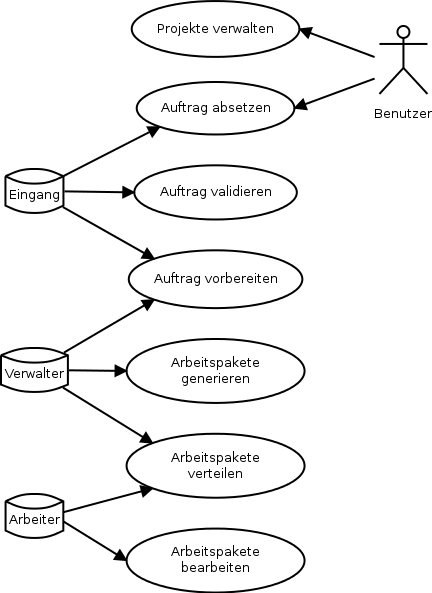
\includegraphics[width=0.7\textwidth]{imageinput/use-case-muss.png}
  \caption{\"Ubersicht Usecases - Kern}
  \label{fig:use-case-muss}
\end{figure}

Wie in \Cref{fig:use-case-muss} gezeigt,
stellt sich der absolute Kern eines CI-Systeme aus relativ wenigen Funktionalitäten zusammen.

Die erste notwendige Funktion stellt die Verwaltung von Projekten \deffeat{projekt-verwalten} dar.
Sind diese dann angelegt, kann man damit beginnen, Aufträge abzusetzen \deffeat{auftrag-absetzen}.
Ist ein Auftrag abgesetzt, so muss seine Richtigkeit sichergestellt werden \deffeat{auftrag-validieren},
danach kann er für die Bearbeitung \deffeat{auftrag-vorbereiten} vorbereitet werden.

Nachdem der Auftrag an sich vorbereitet ist, müssen entsprechend der Build-Matrix \deffeat{auftrag-matrix}
Arbeitspakete generiert werden \deffeat{arbeitspacket-generieren}.
Diese Arbeitspakete werden anschließend verteilt \deffeat{arbeitspacket-verteilen} und abgearbeitet \deffeat{arbeitspacket-abarbeiten}.

Das Abarbeiten der Arbeitspakete sollte in Schritten erfolgen \deffeat{arbeitspackete-schritte},
wobei die grundlegende Art von Arbeitsschritten das Ausführen eines Prozesses \deffeat{arbeitsschritt-prozess} ist.


\subsection{Weiterführende Funktionen}

Nach der Umsetzung des funktionalen Kerns als Basis
k\"onnen nun weiterf\"uhrende Funktionen angelagert werden.
Diese sind nicht zwingend notwendig, tragen jedoch erheblich dazu bei,
informierte Entscheidungen \"uber den Zustand eines Projektes in Integration zu treffen.

\subsubsection{Datensammlung}

Zun\"achst einmal gilt es Datensammlung beim Ablauf eines Arbeitsschritts zu betrachten.
\"Ublicherweise muss zumindest STDOUT/STDERR schon zur Laufzeit festgehalten \deffeat{arbeisschritt-stdio} werden.
Weiterhin besteht  Interesse an statistisch auswertbaren Daten
wie z.B. den Speicherverbrauch \deffeat{arbeitsschritt-stats}.

Nach dem Ausf\"uhren eines Arbeitsschritts fallen interessante Daten an.
Oftmals sorgt zumindest einer der Arbeitsschritte für das Generieren eines ausführbaren Programms.
Dieses sollte sp\"ater auch zur Verf\"ugung gestellt werden \deffeat{arbeitsschritt-artefakt}.
Weiterhin finden sich Test-Resultate in diversen Standardformaten \deffeat{arbeitsschritt-resultate},
wie z.B. JunitXML \cite{jenkins:junitxml} oder \ac{TAP}.

\subsubsection{Arten Arbeitsschritte}

Bei den Arten der Arbeitsschritte gibt es für gew\"ohnlich mehrere M\"oglichkeiten (siehe Kapitel~\ref{chap:ist-analyse}).
Neben den gewohnten Prozess-Schritten (\reffeat{arbeitsschritt-prozess}) sind weitere Arten \"ublich.
Interaktionen mit dem Quellcodemanagement \deffeat{arbeitsschritt-scm} sowie
Schritte implementiert in einer Skript-Sprache \deffeat{arbeitsschritt-script}
stellen weiterf\"uhrende Hilfen dar.

\subsubsection{Verteilung von Arbeitspaketen}

Um \"uberhaupt bis zu den Arbeitsschritten zu kommen,
ist es notwendig, \mbox{Arbeitspakete} zu verteilen \deffeat{arbeitspackete-verteilen}.
Dies soll ein verteilter Prozess sein \deffeat{arbeitspackete-autonome-verteilung},
bei dem die Slaves/Arbeiter aktiv mitwirken k\"onnen.
Eine denkbare Erweiterung w\"are die Möglichkeit, dass Slaves/Arbeiter
die Arbeitspakete mittels kategorischer Filter auswählen \deffeat{arbeitspackete-verteilung-selektiv}.
Beispiele f\"ur diese sind Plattform oder Betriebsumgebung.

\subsubsection{Auftragseingang und Vorbereitung}

%XXX: web hook gosar

Der Auftragseingang kann sich vielseitig gestalten.
Moderne Systeme unterstützen eine Vielzahl von Medien \deffeat{auftrag-eingang-medien},
wie z.B. E-Mail, Web-Hooks, Web-Formulare oder zeitgesteuerte Systeme.

W\"unschenswerte Erweiterungen, welche nicht von existierenden Systemen unterst\"utzt werden,
sind die Anreicherung eines Auftrages um eigene Daten/\"Anderungen.
Besonders hilfreich erscheint hierbei das sogenannte Workdir-diff \deffeat{auftrag-eingang-diff},
welches die aktuellen \"Anderungen eines Entwicklers darstellen.
Dies macht sie besonders n\"utzlich f\"ur den laufenden Entwicklungsprozess.

\subsubsection{Resultatanalyse}

Analyse von Resultaten ist ein vielseitiges Thema,
welches vorwiegend Aufgabe der Erweiterungen sein soll.

In der grundlegend eingebauten Ausf\"uhrung soll zumindest der Erfolg oder Misserfolg
von Auftr\"agen, Arbeitspaketen und Arbeitsschritten feststellbar sein \deffeat{einfache-resultate}.

Die weitergehende Analyse von Ergebnissen soll mittels Erweiterungen behandelt werden.

\subsection{Exemplarische Erweiterungen}

Um die Erweiterbarkeit des Systems aufzuzeigen,
sollen zwei exemplarische Erweiterungen betrachtet werden.
Diese werden hier nur grob umrandet und dann sp\"ater in der Analyse genauer spezifiziert.

Die erste Erweiterung betrachtet vergleichende Analysen von Testergebnissen \deffeat{ext-testing}.
Dabei sollen Entwickler in die Lage versetzt werden,
das Fehlerverhalten eines Programms in verschiedenen Konfigurationen und Auftr\"agen zu vergleichen.
Dies dient zur Vereinfachung der Fehleranalyse.

Die zweite Entwicklung betrachtet ein gänzlich anderes Thema.
Dabei soll das Verhalten einer Version eines Programms
in sehr vielen Kombinationen verst\"andlich gemacht werden \deffeat{ext-analysis}.
Dies soll die Flexibilit\"at des Systems zeigen und
Ideen f\"ur neue Ans\"atze und Werkzeuge bei der Qualit\"atssicherung liefern.


%XXX eventuell spaeter
%\subsection{Vorgaben f. Entwiclungsumgebung}?
%- testen notwendig
%- das system selber ci unterziehen

% %- regeln


\section{Testkriterien}
\label{sec:target:tests}

Dieser Abschnitt beschäftigt sich mit verschiedenen Tests,
die zur Sicherstellung der Funktionalität des Systems notwendig sind.
Dies sind zum einen alle Arten von automatischen Tests,
die auch dazu verwendet werden sollen, das System an sich einer \ac{CI} zu unterziehen
und zum anderen die Manuellen Tests, welche schwer automatisierbare Vorgänge festhalten.


\subsection{Unit-Tests}

Unit-Tests werden verwendet, um die kleinsten Komponenten des Systems zu testen.
Durch ihre starke Koppelung an Implementation und Entwurf,
sind sie w\"ahrend der Kriterien-Findung noch nicht n\"aher bestimmbar.

Sie ergeben sich zum Teil im Entwurf und vorwiegend in
der nachfolgenden Implementation.

\subsection{Funktionale Tests}

Funktionale Tests testen einzelne, funktionale Komponenten des Systems.
Daher entsprechen sie grob den funktionalen Anforderungen und Use-Cases.
%XXX: mehr text

\subsection{Systemtests}

Systemtests testen Kombinationen von funktionalen Komponenten sowie das Komplettsystem.
Im Rahmen dieser Arbeit werden drei Systemtests definiert.


\begin{description}
  \item[Komponentendurchlauf:]
    Der Komponentendurchlauf soll anhand des Ausführens der einzelnen, funktionalen Komponenten aufzeigen,
    ob das Zusammenspiel der Komponenten grunds\"atzlich funktioniert.
  \item[Komplettstystem:]
    Der Test des Komplettsystems soll das komplette CI-System auf einer Testdatenbank starten
    und seine Funktion sicherstellen
  \item[Beispiel Datenanalyse:]
    Das Beispiel Datenanalyse soll die Funktion der Beispielerweiterung für die Datenanalyse sicherstellen
\end{description}

\subsection{manuelle Tests}

Die manuellen Tests umfassen alle Tests,
deren Umsetzung als automatisches Programm erfahrungsgemäß zeitaufwendig,
fehleranfällig und/oder umfangreich ist.
Sie werden deshalb von Hand ausgeführt.

\begin{description}
  \item[Zeitliches Verhalten:]
    Die Beobachtung und Analyse des Zeitverhaltens
    bei wachsender Datenmenge und Auftragsgröße soll Aufschluss über algorithmische Engpässe geben.
  \item[Race-Conditions:]
    Die Beobachtung und Analyse trivialer Race-Conditions
    bei wachsender Nebenl\"aufigkeit soll Probleme bei der Skalierbarkeit aufdecken.
  \item[Verhalten bei Systemfehler:]
      Der Verhaltenstest bei Systemfehlern dient der
    \"Uberpr\"ufung des Verhaltens beim Absturz von Teilkomponenten.
  \item[Große Datenanalyse:]
    Die Große Datenanalyse wird die exemplarischen Erweiterungen mit Datenmengen und Aufgaben,
    welche den Rahmen eines automatischen Tests sprengen überprüfen.
\end{description}


\section{Abgrenzung}
\label{sec:target:abgrenzung}

In dieser Arbeit sollen nur der prototypische Kern eins \ac{CI}-Systems
sowie exemplarische Erweiterungen geschaffen werden.
Somit sind viele Themen, welche für ein produktiv eingesetztes \ac{CI}-System notwendig
sind, nicht weiter zu betrachten.
Benutzer und ihre Rechte sollen nicht betrachtet werden.
Authentifikation und Authorisation sind weitreichende Themengebiete,
die sorgfältig betrachtet werden müssen.
Dies ist neben der Hauptaufgabe nicht im zeitlichen Rahmen unterzubringen.
Außerdem wird kein Wert auf die Benutzeroberfläche gelegt.
Intuitive Benutzerinteraktion ist ein überaus umfangreiches Thema.
Dabei sind auch weiterführende Interaktionen,
wie z.B. Konfiguration der Replikation ausgeschlossen.


\section{Zusammenfassung}
\label{sec:target:zusammenfassung}
%XXX: more text

Die wesentliche Aufgabe ist es, den Kern des \ac{CI}-Systems als Protoyp zu schaffen.
Anschließend sollen weitere Funktionen sowie exemplarische Erweiterungen
auf dieser Basis geschaffen werden.
L\"osungskonzepte f\"ur die einzelnen Komponenten sollen vorgestellt werden,
um anschließend ihre Eigenschaften zu betrachten.

Fokus sind dabei die Interaktionen mit der Datenbank und die Datenoperationen.
Semantik des Systems und das Konsistenz-Verhalten bei Datenbankpartitionierung
sollen betrachtet werden. Erweiterungen zur Datenanalyse sollen ebenfalls nur auf technischer Ebene behandelt werden.

Themen wie Benutzerschnittstellen, Rechteverwaltung und Details
von visueller Komponentenintegration werden dabei nicht betrachtet.
Ziel dieser Arbeit ist die Betrachtung der Kernfunktionen und Erweiterungen auf Datenbank-Ebene.

% zusammenfassung 
%   - im wesentlichen soll \ldots. prototypisch & exemplarisch
%   anhand .. soll ein loesungskonz vorgestellt werden
